
%(BEGIN_QUESTION)
% Copyright 2014, Tony R. Kuphaldt, released under the Creative Commons Attribution License (v 1.0)
% This means you may do almost anything with this work of mine, so long as you give me proper credit

Determine the amount of voltage dropped by each resistor in this circuit, if each resistor has a color code of Brn, Blk, Red, Gld (assume perfectly precise resistance values -- 0\% error):

$$\includegraphics[width=15.5cm]{i01181x01.eps}$$

Also, determine the following information about this circuit:

\begin{itemize}
\item{} Current through each resistor 
\item{} Power dissipated by each resistor
\item{} Ratio of each resistor's voltage drop to battery voltage ($E_R \over E_{bat}$)
\item{} Ratio of each resistor's resistance to the total circuit resistance ($R \over R_{total}$)
\end{itemize}

\underbar{file i01181}
%(END_QUESTION)





%(BEGIN_ANSWER)

Voltage across each resistor = 1.5 V

\vskip 10pt

Current through each resistor = 1.5 mA

\vskip 10pt

Power dissipated by each resistor = 2.25 mW

\vskip 10pt

Voltage ratio = $1 \over 3$

\vskip 10pt

Resistance ratio = $1 \over 3$

%(END_ANSWER)





%(BEGIN_NOTES)

When performing the mathematical analysis on this circuit, there is more than one possible sequence of steps to obtaining the solutions.  Different students in your class may very well have different solution sequences, and it is a good thing to have students share their differing problem-solving techniques before the whole class.

An important aspect of this question is for students to observe the identical ratios (voltage versus resistance), and determine whether or not these ratios are equal by chance or equal by necessity.  Ask your students, "What kind of evidence would prove these ratios were merely equal by chance?"  Setting mathematics aside and viewing this circuit from a purely experimental point of view, ask your students what data could possibly prove these ratios to be equal by chance in this particular case?  Hint: it would only take a single example to prove this!

%INDEX% Electronics review: series and parallel circuits

%(END_NOTES)


